\setcounter{page}{1}
\section*{Zielsetzung}
Im Versuch 401 \emph{Das Michelson-Interferometer} sollen Interferenzerscheinungen beobachtet und zur Bestimmung
relevanter Kenngrößen sichtbaren Lichtes verwendet werden.
\section{Theorie}
\subsection{Interferenz und Kohärenz}
Als Interferenz wird die Überlagerung einer endlichen Menge von Wellenfronten $\vec{E}\ua{k}$ an einem Ort $\vec{r}$ bezeichnet
\begin{equation}
  \vec{E}\ua{ges}\left(\vec{r}\right) = \sum_k \vec{E}\ua{k}\left(\vec{r}\right).
\end{equation}
Zur Beschreibung der Interferenzerscheinungen bei sichtbarem Licht genügt die Vorstellung des Lichtes als elektromagnetische
Welle. Die Intensität $I$ stellt sich hierbei als Betrag des Poyntingvektors $\vec{S}$ dar
\begin{equation}
  I = \left|\vec{S}\right| = \left| \vec{E} \times \vec{H}\right| = const \cdot \vec{E}^2.
\end{equation}
Im Folgenden wird daher eine Betrachtung der elektrischen Komponente des Feldes ausreichen.
Für das zeitliche Mittel der Gesamtintensität $I\ua{ges}$ einer Überlagerung zweier monochromatischer Wellen
\begin{equation}
  \vec{E}\ua{k} = \vec{E}\ua{0}\cos\left(kx - \omega t - \delta\ua{k} \right)
\end{equation}
gilt somit
\begin{equation}
  I\ua{ges} = \frac{const}{t\ua{2}- t\ua{1}}\int_{t\ua{1}}^{t\ua{2}}\left| \vec{E}\ua{1} + \vec{ua{2}} \right|^2 \dif{x} = 2const\vec{E}\ua{0}^2\left[1 + \cos(\delta_2- \delta_1)\right].
\end{equation}
Die Gesamtintensität enthält also neben der Summe der einzelnen Intensitäten einen sogenannten Interferenzterm $\propto \cos(\delta_2-\delta_1)$, der dazu führt, dass
es je nach Phasendifferenz zur Verstärkung bzw. Schwächung der Gesamintensität kommt (konstruktive bzw. destruktive Interferenz). Ist die Phasendifferenz eine
statistische Funktion der Zeit, so liefert eine Mittelung über einen großen Zeitraum die Auslöschung der Intensität. Das Licht wird in diesem Fall als inkohärent
bezeichnet, es kann nicht zur Beobachtung stationärer Interferenzbilder verwendet werden. Kohärenz liegt genau dann vor, wenn sich die Phasen
der einzelnen Wellenfronten jeweils nur um eine konstante Verschiebung $\delta\ua{i}$ voneinander unterscheiden.
Da sichtbares Licht nicht etwa durch gekoppelte Erregerzentren, sondern durch statistisch verteilte Emissionsakte entsteht,
stellt das ausgesandte Licht einer realen Lichtquelle einen endlichen Wellenzug dar
\begin{equation}
  E(x, t) = \int_{-\infty}^{\infty}\tilde{E}(k)\exp\left[ikx \right]\dif{k}.
\end{equation}
Mit $k = \omega/c$.
Ein Wellenpaket ist damit nicht monochromatisch und daher inkohärent. Anschaulich ist klar, dass nach einem hinreichend großen Zeitraum
an einem beliebigen Punkt jede mögliche Phasendifferenz auftaucht und es somit stets zur destruktiven Interferenz kommt. Dennoch
können auch mit endlichen Wellenzügen genügend kleiner Breite Interferenzphänomene beobachtet werden. Das Frequenzspektrum $\tilde{E}(k)$
ist eine statistische Verteilung der Breite $\Delta \omega$ mit Maximum bei $\omega\ua{0}$.
Für die zeitliche Entwicklung der Phasendifferenz $\Delta \varphi$ der Frequenzen $\omega\ua{0} \pm \frac{\Delta \omega }{2}$ gilt
\begin{equation}
  \Delta \varphi = \Delta \omega \cdot t.
\end{equation}
Nach der sogenannten Kohärenzeit $\tau$ tritt weitesgehend jede mögliche Phasendifferenz zwischen $0$ und $2\pi$ auf
\begin{equation}
  2\pi = \Delta \omega \tau \quad \Leftrightarrow \quad \tau = \frac{2\pi}{\Delta \omega}.
\end{equation}
Da ein großer Teil der auftauchenden Frequenzen innerhalb der Breite $\Delta \omega$ angesiedelt sind, können innerhalb der Kohärenzzeit
bzw. Kohärenzlänge $l = c \tau$ (für Laser $l$ im Bereich $\si{\kilo\meter}$) Interferenzeffekte beobachtet werden.

\subsection{Funktion des Michelson-Interferometers}
\begin{figure}
  \centering
  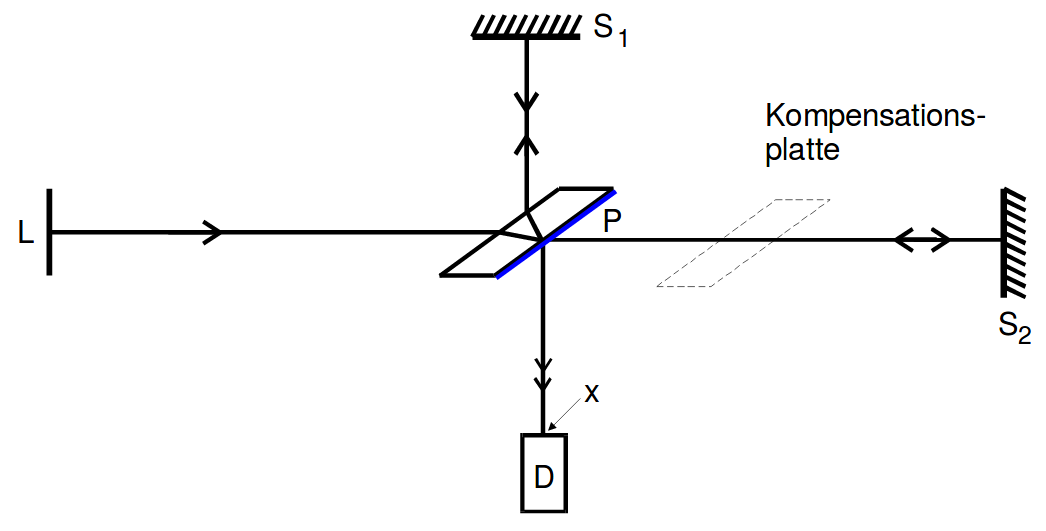
\includegraphics[width = 0.7\textwidth]{table/michelson.png}
  \caption{Schematischer Aufbau des Michelsoninterferometers\cite{anleitung401}.}
  \label{fig: michelson}
\end{figure}
Der prinzipielle Aufbau eines Michelson-Interferometers ist in Abbildung \ref{fig: michelson} dargestellt. Um kohärente Lichtbündel in einem Detektor $D$ miteinander
interferieren zu lassen wird das Licht einer Quelle $L$ mittels eines semipermeablen Spiegels $P$ augeteilt, sodass zwei Teilbündel die unterschiedlichen
Wege $\overline{PS_1PD}$ und $\overline{PS_2PD}$ nehmen. Da das Licht, das zum Spiegel $S_1$ gelangt insgesamt dreimal durch das Material des Spiegels $P$ gebrochen
wird, ist es notwendig zwischen $P$ und $S_2$ eine Kompensationsplatte mit gleichen optischen Eigenschaften wie $P$ zu stellen. Sind nun beide
Lichtwege exakt gleich lang, kommt es wegen des $\pi$ Phasensprungs des $S_2$-Bündels bei der Reflexion an $P$ zur Auslöschung der Gesamtamplitude im Detektor.
Wird der Abstand einer der beiden Spiegel $S\ua{i}$ um die Strecke $d$ varriert, entsteht ein Gangunterschied von $2d$ zwischen den beiden Teilwellen, was
folgenden Ansatz für die Ortsabhängigkeit der elektrischen Feldamplitude motiviert
\begin{equation}
  E\ua{1} = E\ua{0}\exp\left[ikx \right], \quad E\ua{1} = E\ua{0}\exp\left[ikx +2d + \pi \right].
\end{equation}
Für die Intensität als Funktion der Verschiebung $d$ gilt somit
\begin{equation}
  I(d) =  2const E\ua{0}^2\left[1 + \cos\left(\frac{2\pi}{\lambda}2d + \pi  \right)\right].
\end{equation}
Eine Verschiebung um Vielfache von $\lambda / 2$ führt also zu der selben Intensität. Wird der Spiegel um eine Distanz $\Delta d$ verschoben, so können
$z$ Intensitätsmaxima im Detektor nachgewiesen werden
\begin{equation}
  \Delta d = z\frac{\lambda}{2} \quad \Leftrightarrow \quad \lambda = \frac{2 \Delta d}{z}.
  \label{eq: maxima_wellenlänge}
\end{equation}
Das Michelson-Interferometer kann somit zur Bestimmung der Wellenlänge des Lichtes der Quelle $L$ benutzt werden. Sind die verwendeten
Lichtstrahel divergent, treten darüber hinaus Intensitätsmaxima als Funktion des Winkels $\alpha\ua{k}$ zwischen Einfallslot und Ausfallswinkel an den Spiegeln $S\ua{i}$
auf. Das Interferenzmuster entspricht in diesem Fall konzentrischen Ringen.\\
Um die Differenz zweier Brechungsindices $\Delta n$ zu bestimmen, wird in den Aufbau nach Abbildung \ref{fig: michelson} zwischen $P$ und einem der Spiegel $S\ua{i}$ eine
mit Gas gefüllte Messzelle der Breite $b$ integriert. Ist der Brechungsindex dieses Gases um $\Delta n$ größer als jener der Umgebung,
tritt ein Gangunterschied von $\Delta n b$ auf. Wird ausgehend von einem Vakuum der Gasdruck allmählich erhöht, werden $z$ Intensitätsmaxima am Detektor
registriert
\begin{equation}
  b \Delta n = z\frac{\lambda}{2} \quad \Leftrightarrow \quad \Delta n = \frac{z \lambda}{2b}.
  \label{eq: maxima_brechungsindex}
\end{equation}
